%
% xtal formulas
% @author Tobias Weber <tweber@ill.fr>
% @date 13-jul-2018
% @license see 'LICENSE' file
%

% ------------------------------------------------------------------------------------------------------------------------------------
\section{Fractional Coordinates}

\begin{center}
	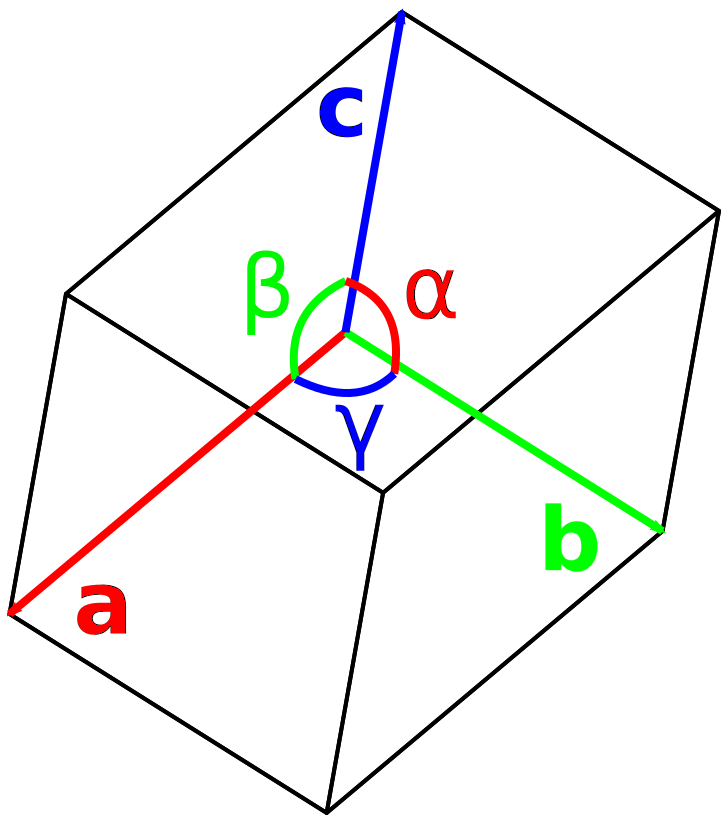
\includegraphics[width = 0.2 \textwidth]{figures/cell}
\end{center}

\subsection*{Basic Properties}

From the cosine theorem we get:
\begin{equation} \left< a | b \right > = ab \cos \gamma, \label{ab} \end{equation}
\begin{equation} \left< a | c \right > = ac \cos \beta, \label{ac} \end{equation}
\begin{equation} \left< b | c \right > = bc \cos \alpha. \label{bc} \end{equation}


\subsection*{Basis Vectors}

We first choose $\left| a \right>$ along $x$,
\begin{equation} \boxed{ \left| a \right> = \left( \begin{array}{c} a_1 = a \\ 0 \\ 0 \end{array} \right), } \label{avec} \end{equation}
$\left| b \right>$ in the $xy$ plane,
\begin{equation} \left| b \right> = \left( \begin{array}{c} b_1 \\ b_2 \\ 0 \end{array} \right), \end{equation}
and $\left| c \right>$ in general:
\begin{equation} \left| c \right> = \left( \begin{array}{c} c_1 \\ c_2 \\ c_3 \end{array} \right). \end{equation}


Inserting $\left| a \right>$ and $\left| b \right>$ into Eq. \ref{ab} gives:

\begin{equation} \left< a | b \right > = a_1 b_1 = ab \cos \gamma, \end{equation}
\begin{equation} b_1 = b \cos \gamma. \end{equation}


Using the cross product between $\left| a \right>$ and $\left| b \right>$, we get:
\begin{equation} \left\Vert \left| a \right> \times \left| b \right> \right\Vert =
	\left\Vert \left( \begin{array}{c} 0 \\ 0 \\ a_1 b_2 \end{array} \right) \right\Vert =
	ab \sin \gamma, \label{crossab}
\end{equation}
\begin{equation} b_2 = b \sin \gamma, \end{equation}
\begin{equation} \boxed{ \left| b \right> = \left( \begin{array}{c} b \cos \gamma \\ b \sin \gamma \\ 0 \end{array} \right). } \label{bvec} \end{equation}


Inserting $\left| a \right>$ and $\left| c \right>$ into Eq. \ref{ac} gives:

\begin{equation} \left< a | c \right > = a_1 c_1 = ac \cos \beta, \end{equation}
\begin{equation} c_1 = c \cos \beta. \end{equation}



Inserting $\left| b \right>$ and $\left| c \right>$ into Eq. \ref{bc} gives:

\begin{equation} \left< b | c \right > = b_1 c_1 + b_2 c_2 = bc \cos \alpha, \end{equation}
\begin{equation} b \cos \gamma \cdot c \cos \beta + b \sin \gamma \cdot c_2 = bc \cos \alpha, \end{equation}
\begin{equation} c_2 = \frac{c \cos \alpha - c \cos \gamma \cos \beta}{\sin \gamma}. \end{equation}



The last component, $c_3$, can be obtained from the vector length normalisation, $ \left< c | c \right> = c^2 $:
\begin{equation} \left< c | c \right > = c_1^2 + c_2^2 + c_3^2 = c^2, \end{equation}
\begin{equation} c_3^2 = c^2 - c_1^2 - c_2^2, \end{equation}
\begin{equation} c_3^2 = c^2 \left[1 - \cos^2 \beta - \left(\frac{\cos \alpha - \cos \gamma \cos \beta}{\sin \gamma} \right)^2 \right], \end{equation}
\begin{equation} \boxed{ \left| c \right> = \left( \begin{array}{c}
	c \cdot \cos \beta \\
	c \cdot \frac{\cos \alpha - \cos \gamma \cos \beta}{\sin \gamma} \\
	c \cdot \sqrt{ 1 - \cos^2 \beta - \left(\frac{\cos \alpha - \cos \gamma \cos \beta}{\sin \gamma} \right)^2 }
\end{array} \right). } \label{avec} \end{equation}



The crystallographic $A$ matrix, which transforms real-space fractional to lab coordinates (A), is formed with the basis vectors in its columns:
\begin{equation}
	A = \left(
		\begin{array}{ccc}
			\left| a \right> & \left| b \right> & \left| c \right>
		\end{array}
	\right).
\end{equation}
The $B$ matrix, which transforms reciprocal-space relative lattice units (rlu) to lab coordinates (1/\AA), is:
\begin{equation} B = 2 \pi A^{-t}, \end{equation}
where $-t$ denotes the transposed inverse.
The metric tensor corresponding to the coordinate system defined by the $B$ matrix is:
\begin{equation} \left(g_{ij}\right) = \left<\bm{b_i} | \bm{b_j} \right> = B^T B, \end{equation}
where the reciprocal basis vectors $\left| \bm{b_i} \right>$ form the columns of $B$.


\subsection*{Example: Lengths and Angles in the Reciprocal Lattice}
Having a metric makes it straightforward to calculate lengths and angles.
The length of a reciprocal lattice vector $\left| G \right>$ seen from the lab system is (in 1/\AA{} units):
\begin{equation}
	\left\Vert \left< G | G \right> \right\Vert = \sqrt{\left< G | G \right>} = \sqrt{G_i G^j} = \sqrt{g_{ij} G^i G^j}.
\end{equation}
The angle $\theta$ between two Bragg peaks $\left| G \right>$ and $\left| H \right>$ is given by their dot product:
\begin{equation}
	\frac{\left< G | H \right>}{\left\Vert \left< G | G \right> \right\Vert \cdot \left\Vert \left< H | H \right> \right\Vert} = \cos \theta,
\end{equation}
%\begin{equation}
%	\frac{G_i H^j }{\left\Vert \left< G | G \right> \right\Vert \cdot \left\Vert \left< H | H \right> \right\Vert} = \cos \theta,
%\end{equation}
\begin{equation}
	\frac{g_{ij} G^i H^j }{\sqrt{g_{ij} G^i G^j} \sqrt{g_{ij} H^i H^j}} = \cos \theta.
\end{equation}


% ------------------------------------------------------------------------------------------------------------------------------------




% ------------------------------------------------------------------------------------------------------------------------------------
\section{TAS Angles and Scattering Triangle}
\begin{figure}
\begin{center}
	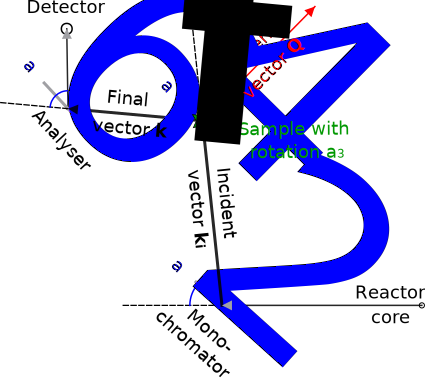
\includegraphics[width = 0.5 \textwidth]{figures/tas}
	\hspace{1.5cm}
	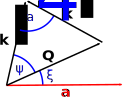
\includegraphics[trim=0 -2cm 0 0, width=0.25\textwidth]{figures/triangle}
\end{center}
\caption{Triple-axis layout and scattering triangle.}
\end{figure}

\subsection*{Monochromator Angles $a_1$, $a_2$ and Analyser Angles $a_5$, $a_6$}

The monochromator (and analyser) angles follow directly from Bragg's equation:
\begin{equation} 2 d_{m,a}\sin a_{1,5} = n \lambda_{i,f}, \end{equation}
\begin{equation} 2 k_{i,f} \sin a_{1,5} = 2 \pi n / d_{m,a}, \end{equation}
\begin{equation} \boxed{ a_{1,5} = \arcsin \left( \frac{\pi n}{d_{m,a} \cdot k_{i,f}} \right). } \end{equation}

Fulfilling the Bragg condition, the angles $a_2$ and $a_6$ are simply: $a_{2,6} = 2 \cdot a_{1,5}.$


\subsection*{Scattering Angle $a_4$}

\begin{equation} \left| Q \right> = \left| k_i \right> - \left| k_f \right> \\ \end{equation}
\begin{equation} \left< Q | Q \right> = \left( \left< k_i \right| - \left< k_f \right| \right) \cdot \left( \left| k_i \right> - \left| k_f \right> \right) \end{equation}
\begin{equation} \left< Q | Q \right> = \left< k_i | k_i \right> + \left< k_f | k_f \right> - 2 \left< k_i | k_f \right> \end{equation}
\begin{equation} Q^2 = k_i^2 + k_f^2 - 2 k_i k_f \cos a_4 \end{equation}
\begin{equation} \boxed{ a_4 = \sigma_s \cdot \arccos \left( \frac{k_i^2 + k_f^2 - Q^2}{2 k_i k_f} \right) } \end{equation}

The sign of $a_4$ is given by the sample scattering sense $\sigma_s = \pm 1$.



\subsection*{Rocking Angle $a_3$}

\begin{equation} \boxed{ a_3 = 180^{\circ} - \left( \psi + \xi \right) } \end{equation}


\subsubsection*{Angle $\psi$}
Angle $\psi$ between $\left| k_i \right>$ and $\left| Q \right>$, in units of \AA{}$^{-1}$, as before:
\begin{equation} \left| k_f \right> = \left| k_i \right> - \left| Q \right> \end{equation}
\begin{equation} \left< k_f | k_f \right> = \left( \left< k_i \right| - \left< Q \right| \right) \cdot \left( \left| k_i \right> - \left| Q \right> \right) \end{equation}
\begin{equation} \left< k_f | k_f \right> = \left< k_i | k_i \right> + \left< Q | Q \right> - 2 \left< k_i | Q \right> \end{equation}
\begin{equation} k_f^2 = k_i^2 + Q^2 - 2 k_i Q \cos \psi \end{equation}
\begin{equation} \boxed{ \psi = \sigma_s \cdot \arccos \left( \frac{k_i^2 + Q^2 - k_f^2}{2 k_i Q} \right) } \end{equation}


\subsubsection*{Angle $\xi$}
Angle $\xi$ between $\left| Q \right>$ and orientation vector $\left| a \right>$ (i.e. $ax$, $ay$, $az$), in units of rlu:
\begin{equation} \xi = \sigma_{\mathrm{side}} \cdot \arccos \left( \frac{ \left< Q | a \right> }{ \sqrt{\left< Q | Q \right>} \sqrt{\left< a | a \right>} } \right) \end{equation}
\begin{equation} \boxed{ \xi = \sigma_{\mathrm{side}} \cdot \arccos \left( \frac{ Q^i g_{ij} a^j }{ \sqrt{Q^i g_{ij} Q^j} \sqrt{a^i g_{ij} a^j} } \right) } \end{equation}

The sign, $\sigma_{\mathrm{side}}$, of $\xi$ depends on which side of the orientation vector $\left| a \right>$ the scattering vector $\left| Q \right>$ 
is located. The sign can be found by calculating the (covariant) cross product of $\left| a \right>$ and $\left| Q \right>$ to give an out-of-plane vector 
which can be compared with the given scattering plane up vector.


\paragraph*{Special case}
Special case for cubic crystals, $g_{ij} = \delta_{ij} \cdot \left( 2\pi / a \right)^2$:
\begin{equation} \xi = \sigma_{\mathrm{side}} \cdot \arccos \left( \frac{ Q_i a^i }{ \sqrt{Q_i Q^i} \sqrt{a_i a^i} } \right) \end{equation}
% ------------------------------------------------------------------------------------------------------------------------------------
